\chapter{Research Plan}
\label{chapter:plan}
% **************************** Define Graphics Path **************************
\ifpdf
    \graphicspath{{Chapter4/Figs/Raster/}{Chapter4/Figs/PDF/}{Chapter4/Figs/}}
\else
    \graphicspath{{Chapter4/Figs/Vector/}{Chapter4/Figs/}}
\fi

This section describes the goals for this thesis step by step and how the work is organised.
The general subject of this thesis is the efficient exploitation of asymmetric systems.

\section{Exploring the maturity of asymmetric systems}
\label{sec:asymmetric}
In this step of the thesis, we evaluate for the first time the suitability of currently available mobile asymmetric multi-core platforms for general purpose computing. 
This part of work has been implemented and is submitted to an international conference being currently under review.
First, we demonstrate that out-of-the-box parallel applications do not run efficiently on asymmetric multi-cores. Fully exploiting the computational power of these processors is challenging as the asymmetry in the system can lead to load imbalance, undermining the scalability of the parallel application. Consequently, only applications that incorporate user-defined load balancing mechanisms can benefit immediately from asymmetric multi-cores.

When load-balancing techniques are not included in the original application, we evaluate alternative solutions that, without relying on the programmer, can leverage the opportunities that asymmetric systems offer. In particular, we evaluate a state of the art dynamic scheduler at the Operating System (OS) level that is aware of the characteristics of each core type~\cite{samsung}. This scheduler effectively exploits the system by running high CPU utilization processes on the big cores and low CPU utilization processes on the little cores.

An alternative to tackle the challenges of asymmetric multi-cores consists in transferring the responsibility of managing the parallel workload from the OS to the runtime system. Recent task-based programming models rely on an advanced runtime system to dynamically schedule tasks~\cite{Ayguade:TPDS2009, OpenMP4.0:Manual2013, OmpSs_PPL11, Zuckerman:EXADAPT2011, Bauer.2012.SC, Vandierendonck:PACT2011, Vandierendonck:Hyperq}. By allowing the programmer to specify the inter-task dependencies, these programming models rely on the runtime system for the dynamic scheduling of tasks to achieve load balancing.

More precisely, this part of work aims to evaluate three different scenarios of parallel execution when transferring the scheduling responsibility at different levels of the software stack:
\begin{itemize}
\item \textit{Static Threading:} the scheduling responsibility is on the application level. The implementation of the application performs the scheduling.
\item \textit{OS Scheduling (GTS):} the operating system is responsible for performing the scheduling. Specifically we use the Global Task Scheduler (GTS) provided by ARM that is aware of the characteristics of the asymmetric system.
\item \textit{Task-based:} the runtime system is responsible for the efficient scheduling. Specifically we use applications written with the OmpSs programming model~\cite{OmpSs_PPL11}~\cite{OmpSs} and the runtime is unaware of the platform.
\end{itemize}


\section{Scheduling policies for asymmetric systems}
\label{sec:scheduling}
We aim to improve the efficiency of the runtime system and make it aware of the underneath architecture.
This is the motivation for the proposed scheduling techniques that take into account the asymmetry of the platform.
We implement different scheduling policies in the runtime system of the OmpSs programming model as an approach to increase performance and energy efficiency.
Even though task-based programming models is a powerful mechanism, the efficient mapping of ready tasks to different types of cores on an asymmetric system remains a challenge.
Task-based parallel applications expose different characteristics that can affect the total application duration such as complex task dependency graphs (TDGs) with long critical paths or different levels of task cost variability.
These characteristics influence researchers to develop smart scheduling techniques within a task-based programming model and accelerate the overall application.
The criticality-aware schedulers detect the critical tasks of an application and increase performance by running critical tasks on fast cores. 
Unlike the previous works mentioned in Section~\ref{sec.relwork_critical}, our schedulers, do not rely on profiling information and are evaluated on real scientific applications.
%Some previous works~\cite{DCPS, LDCP, HEFT, CrPathDup} tackled this issue using static scheduling over the whole TDG to statically map tasks to processors on a heterogeneous system. 
%However, they required the knowledge of profiling information and most of them were evaluated on synthetic randomly-generated TDGs. 

In this work, we propose three novel dynamic task schedulers that detect the critical tasks of the TDG. 
The purpose of these scheduling techniques is to separate the tasks into two groups: critical and non-critical.
To to so, these schedulers maintain two ready queues: the critical queue and the non-critical queue.
When a task becomes ready, the scheduler decides according to the policy whether it is critical or not.
If the task is critical it is inserted in the critical ready queue while if the task is non-critical it is inserted in the non-critical ready queue.
Each time a processor becomes idle, it retrieves a task from one of the ready queues to execute.
In our scheduling approaches, the fast cores of the system always check for ready tasks in the critical queue and the slow cores look for tasks in the non-critical queue.
As a result, fast cores execute critical tasks and slow cores execute the non critical tasks.
In the following sections we describe in more detail the different scheduling policies for asymmetric systems.
A journal paper has been authored and is currently under peer review.

\subsection{Criticality-Aware Task Scheduler}
\label{sec:cats}
The first proposed scheduling algorithm generally applies to task-based programming models supporting task dependencies, but for simplicity we explain it in the context of the OmpSs programming model.
This part of work has been already carried out and is published in the International Conference of Supercomputing (ICS) in June 2015~\cite{Chronaki:ICS2015}.

The Criticality-Aware Task Scheduler (CATS)~\cite{Chronaki:ICS2015} uses bottom-level longest-path priorities and consists of three steps:
\begin{itemize}
 \item{\textit{Task prioritization}: when a task is created and added to the task graph, it is assigned a priority and the priority of the rest of tasks in the graph is updated accordingly.}
 \item{\textit{Task submission}: when a task becomes \textit{ready}, i.e., all its predecessors finished their execution, it is submitted to a \textit{ready queue}. At this point, the algorithm decides whether the task is considered \textit{critical} or \textit{non critical}. The task is then inserted in the corresponding ready queue: tasks in the \textit{critical ready queue} will be executed by fast cores, and tasks in the \textit{non-critical ready queue} will be executed by slow cores.}
 \item{\textit{Task-to-core assignment}: when a core becomes idle, it tries to retrieve a task from its corresponding ready queue to execute it. If the queue is empty, it might try to steal from the other queue depending on the work stealing policy. Currently, we support two work stealing mechanisms: \textit{simple} work stealing, i.e., fast cores can steal from slow cores; and \textit{bi-directional} (\textit{2DS}) work stealing, i.e., both types can steal from the other. The default policy is \textit{simple}.}
\end{itemize}

These steps are performed dynamically and potentially in parallel in different cores. This means that while some tasks are being prioritized, previously created tasks may be submitted, and others assigned to available cores or executed.

To give an overview of the scheduling process, Figure~\ref{botlevels} shows a scheme of the operation of CATS. In the TDG on the left, each node represents a task and each edge of the graph represents a dependency between two tasks. The number inside each node is the \textit{bottom level} of the task: the length of the longest path in the dependency chains from this node to a leaf node. The priority of a task is given by its bottom level. The pattern-filled nodes indicate tasks that are considered critical. The number outside each node is the task id and is used in the text to refer to each task. Critical tasks are inserted in the critical queue, and non-critical tasks to the non-critical queue. The insertion is ordered with the highest priorities at the head of the queue and the lowest priorities at the tail. Slow cores retrieve tasks from the head of the non-critical queue and fast cores from the critical queue. The following sections describe these scheduling steps in more~detail.


\begin{figure}[t]
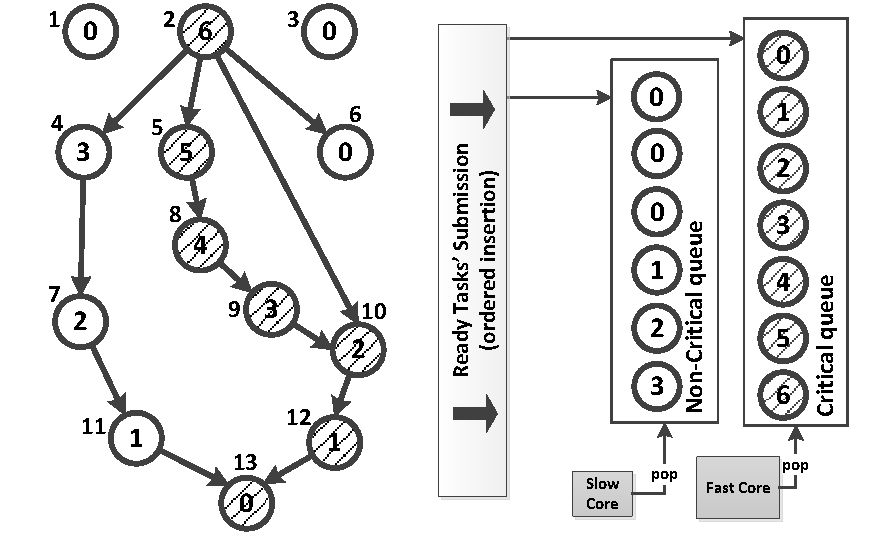
\includegraphics[width=0.6\columnwidth]{Figs/fig_1.pdf} 
\centering
\caption{Task submission with CATS. Nodes are marked with the \textit{bottom level} of each task. Pattern-filled nodes mark the critical tasks.}
\label{botlevels}
\end{figure}


\subsection{Critical Path Scheduler}
\label{sec:cpath}
The Critical Path scheduler (CPATH) dynamically detects the critical path of the TDG.
Like CATS, CPATH separates tasks into two groups: critical and non-critical tasks.
The detected critical tasks are executed by the fast cores in the system and non-critical tasks are executed by slow cores.
The difference with CATS is the algorithm for critical path detection.
CPATH takes into account the task execution time, about which CATS is unaware.
To do so, CPATH implements a more complex and accurate critical path detection algorithm that takes into account task execution time.

CPATH scheduler consists of three steps:
\begin{itemize}

\item \textit{Task prioritization}: this step takes place when a task is finishing its execution (task completion). This is different than CATS since at the end of a task execution the algorithm may record the task execution time (task cost).
%might track a new (unknown) task cost. 
According to the discovered task cost CPATH assigns priorities to tasks by traversing the TDG from top to bottom.

 \item{\textit{Task submission}: when a task becomes \textit{ready}, it is submitted to a \textit{ready queue}. At this point, CPATH decides whether or not the task is \textit{critical} and inserts it in the corresponding ready queue. This step has only slight implementation differences with CATS.}

 \item{\textit{Task-to-core assignment}: this step is identical to CATS and supports the same work stealing mechanisms.}
\end{itemize}
\begin{figure}[tr]
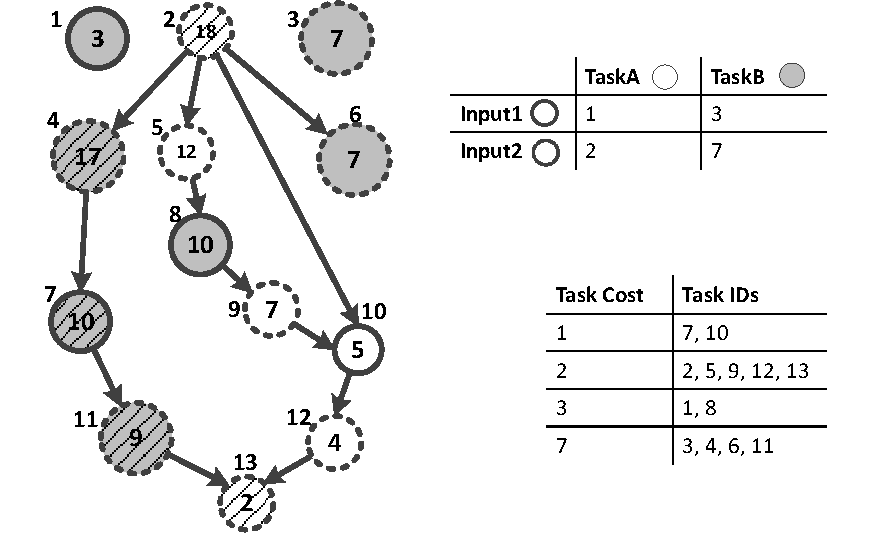
\includegraphics[width=0.6\columnwidth]{Figs/cpath_priorities.pdf} 
\centering
\caption{Priority assignment taking into account the task costs. Task costs are assumed known and are shown in the tables.}
\label{cpath}
\vspace{-0.5cm}
\end{figure}
Figure~\ref{cpath} is used to describe the priority assignment with CPATH.
The specific TDG contains tasks of two different types and two different input sizes.
Node color shows the different task types and the outline of the circle (dashed or solid) shows the different input sizes.
The upper table in Figure~\ref{cpath} indicates the execution time of the tasks according to their type and input size.
The algorithm assumes that task instances of the same type with the same input size have the same (or very similar) execution time.
To track this information, CPATH discovers the cost of every possible task type-input size duple (tt-is duple) that appears on the TDG.
The numbers inside the nodes show the bottom cost-based priorities that CPATH assigns. We define the \textit{bottom cost} of a node on a directed acyclic graph as the maximum estimated time in the dependency chains from this node to a leaf node.The numbers outside the nodes show their task ID.


\subsection{Hybrid Criticality Scheduler}
\label{sec:hybrid}
The Hybrid Criticality Scheduler (HYBRID) is a combination of the CATS and CPATH scheduling policies.
HYBRID keeps the simplicity of the implementation of CATS and introduces the task execution time only if available.
This results in an efficient low-overhead scheduler that computes the critical path of a TDG more faithfully than CATS and with lower overheads than CPATH.
This section describes HYBRID through its relation to CATS and CPATH described in Sections~\ref{sec:cats} and~\ref{sec:cpath}. 
We focus our description on the task prioritization, since task submission and task-to-core assignment for HYBRID are identical to CPATH.

As shown, CPATH computes priorities on task completion. 
The algorithm for priority computation is an expensive operation and is in the critical path of the execution:
on task completion the core becomes available but the start of the next task is delayed by priority computation.
Also, when multiple cores are completing tasks, there will be contention on accessing the TDG for priority computation.
On the other hand, CATS computes priorities during task creation.
The computation of priorities during task creation is more efficient because, unless there is nested parallelism, one core creates all tasks
and therefore there is no contention on priority computation. The downside is that there is potentially less information available 
on task execution time on task creation, as some task type may have not been executed yet at the time all tasks are created.

When comparing CPATH and HYBRID schedulers their logical operation is similar.
However the difference in their implementation may result in different task priorities potentially leading to different schedules.
For applications with small TDGs, HYBRID may not be able to compute an accurate critical path because task creation does not overlap with a sufficient amount of task exits.
Therefore, task execution information will not be available during priority computation and HYBRID will prioritize based on bottom-level priorities (like CATS).
If the application has a large TDG and task creation overlaps with a sufficient amount of task exits, HYBRID will use bottom-cost priorities.

\section{Runtime thread migration mechanisms}

The asymmetry-aware scheduling policies may increase the runtime overheads.
Especially when the runtime operations are executed by the fast cores of the system, preventing them from executing user tasks, the runtime activity can create a bottleneck at the task execution.
This is the motivation for reserving one core responsible for the execution of the runtime activities.
This way the rest of the cores will be devoted for the uninterrupted task execution.
The following subsections describe our motivation and background of this work as well as the current software modifications.
\subsection{Motivation}
\begin{figure}[t]
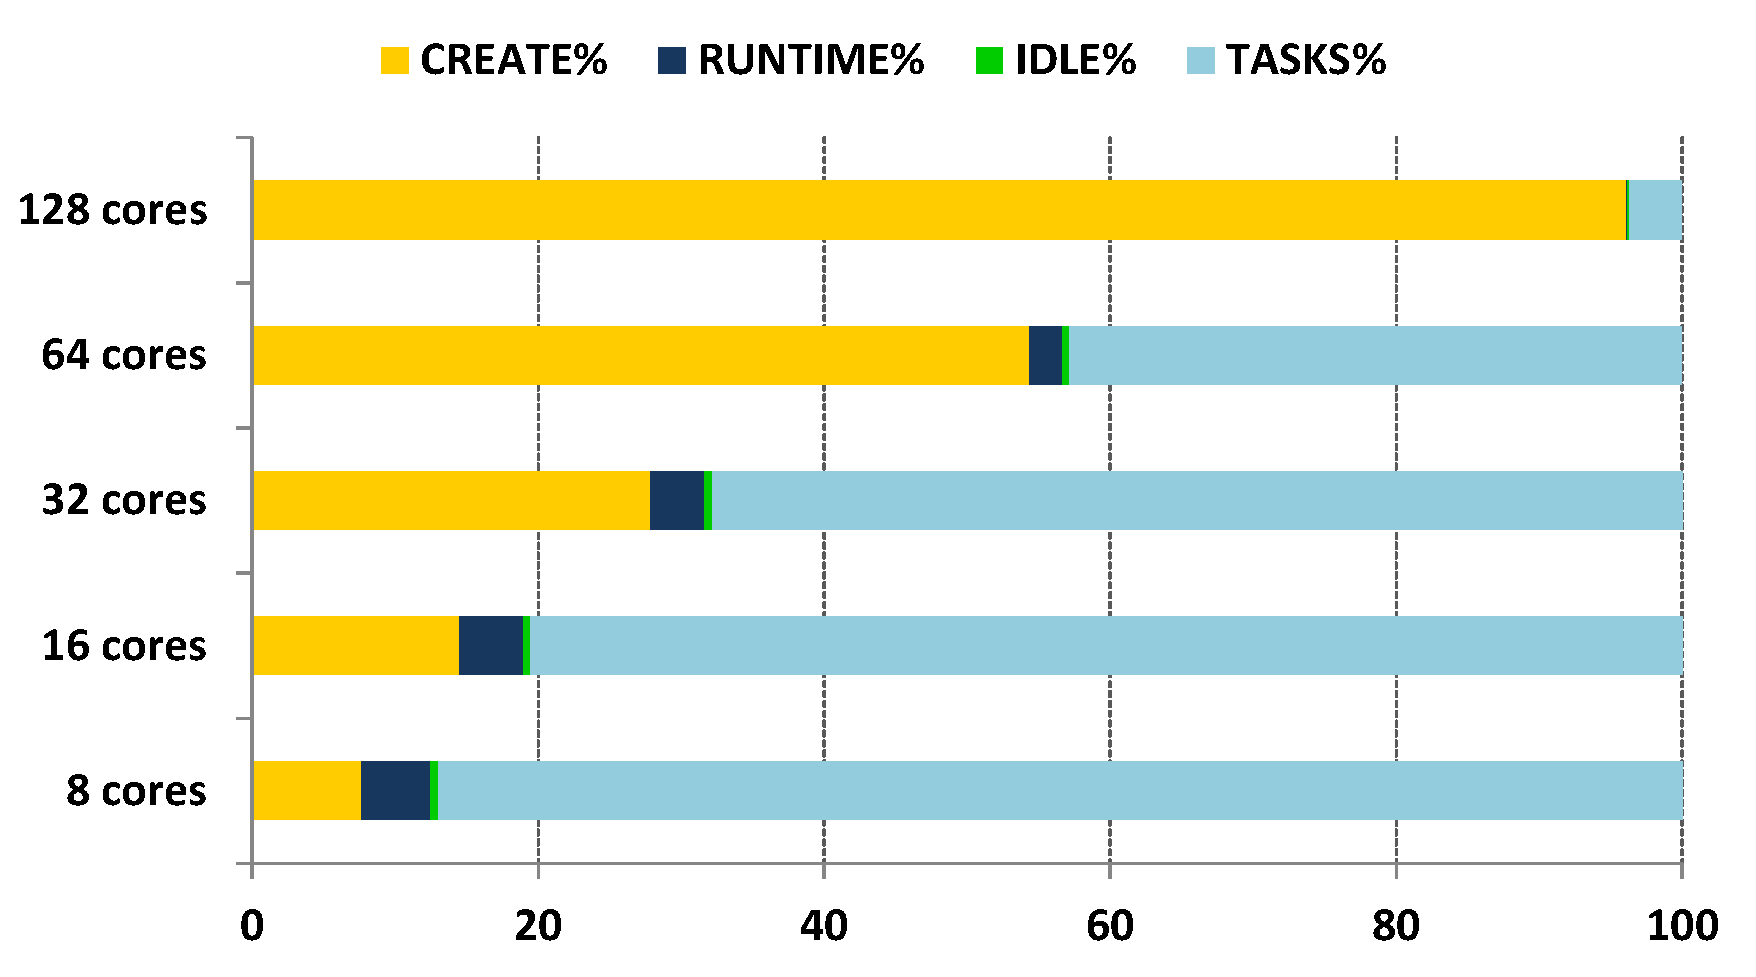
\includegraphics[width=0.6\columnwidth]{Figs/master_thread.pdf} 
\centering
\caption{Activity breakdown of the master thread when executing a parallel application.}
\label{master_activity}
\end{figure}
Task creation is a bottleneck for most applications especially when using smart scheduling policies like the ones we described.
Figure~\ref{fig:master_activity} shows the runtime activity of the master thread during the execution of the Cholesky benchmark on 8, 16, 32, 64 and 128 cores.
Each one of the series represents a different runtime overhead from the ones described above.
CREATE represents the \textit{Creation} step, 
RUNTIME refers to the \textit{Finish} step, IDLE shows the master thread's idle time and the TASKS is the time spent on task execution. 
The percentage of time spent on task creation is increasing as we increase the number of cores.
This is because the creation overhead is static so the more we reduce the application's execution time by adding resources the more important this step becomes in terms of execution time.
On the other hand, the task execution time percentage is decreased as we increase the number of cores because the computational activity is being shared among more resources.
The RUNTIME decreases as we increase the number of cores because this activity is also shared among the resources.

Our motivation for this work is the bottleneck introduced by task creation (CREATION) as shown in Figure~\ref{fig:master_thread}.
We implement a runtime proposal that decouples this piece of the runtime and accelerates it on a specialized hardware resulting in higher performance.

\subsection{Background}

Once again, OmpSs programming model offers the most appropriate environment for exploring this heuristic.
Like OmpSs, task-based parallel programming models\cite{OpenMP4.0:Manual2013},\cite{OmpSs_PPL11}, \cite{OmpSs},  are widely used to facilitate the programming of parallel codes for multi-core systems.
These programming models offer annotations that the programmer can add to the application's sequential code. 
By adding these annotations, the programmer decomposes the application into \textit{tasks} and specifies the input and output data dependencies between them. 
A compiler is responsible to translate the annotations into code by adding calls to the programming model's runtime system. 
The runtime system consists of software threads and is responsible for the efficient execution of the tasks with respect to the data dependencies as well as the availability of resources.
\begin{lstlisting}[float, emph={void,if,return,non_critical_queue, critical_queue,not,true,and,break}, captionpos=b, caption={Compiler generated pseudo-code equivalence for task annotation.},label=task_clause, emph={[2]mat}, emphstyle={[2]}, aboveskip={0\baselineskip}, frame=tb, belowskip={0\baselineskip}]
     ...
  //task_clause
  memalloc(&task, args, size);
  createTask(deps, task, parent, taskData);
     ...
\end{lstlisting}

When the compiler encounters one task annotation in the code, it transforms it to the pseudo-code shown in Listing~\ref{task_clause}.
\texttt{Memalloc} is performing the memory allocation for the task and its arguments.
Next is a runtime call, which is the createTask, responsible for the linking of the task with the runtime system.
At this point a task is considered \textit{created} and below are the three possible states of a task inside the runtime system:
\begin{itemize}
\item \textit{Created:} A task is initialized with the appropriate data and function pointers and it is inserted in the Task Dependency Graph (TDG). The insertion of a task in the TDG implies that the data dependencies of the tasks have been identified and the appropriate data structures have been created and properly initialized. 
\item \textit{Ready:} When all the data dependencies of a created task have been satisfied, the task is ready and it is inserted in the \textit{ready queue} where it waits for execution. 
\item \textit{Finished:} When a task has finished execution and has not been deleted yet.
\end{itemize}

The runtime system creates and manages the software threads for the execution of the tasks. 
Typically one software thread is being bound to each core. 
One of the threads is the \textit{master thread}, and the rest are the \textit{worker threads}. 
The master thread starts executing the code of Listing~\ref{task_clause} sequentially. 
The allocation of the task takes place first.
What follows is the task creation, that includes the analysis of the dependencies of the created task and the connection to the rest of the existing dependencies.
Then, if there are no task dependencies, which means that the task is ready, the task is also inserted in the ready queue and waits for execution.

Listing~\ref{taskCreation} shows the pseudo-code for the task creation step within the runtime.
The \texttt{createTask} function is first initializing the task by copying the corresponding data to the allocated memory as well as connecting the task to its parent task (\texttt{initAndSetupTask}).
After this step, the task is ready to be inserted in the TDG; this is done by the \texttt{insertToTDG} function.
This function takes as arguments a list with all the memory addresses that are to be written or read by the task (\texttt{dList}), and the task itself.
If for a task the \texttt{dList} is empty, this means that there are no memory addresses that need to be tracked during the execution; thus, the task is marked as \textit{ready} by inserting it in the \textit{ready queue} (\texttt{rQueue\_submission}).
Each entry of \texttt{dList} contains the actual memory address as well as the access type (read, write or read-write).
The runtime keeps a unified dependency tracking structure (\texttt{depMap}) where it stores all the tracked memory addresses together with their writer and reader tasks.
For each item in the \texttt{dList} the runtime searches for an existing representation inside the \texttt{depMap}.
If the memory address of an entry of the \texttt{dList} is not represented in the \texttt{depMap}, it is being added;
if the address of a \texttt{dList} item belongs to the \texttt{depMap}, this means that a prior task has already referred to this memory location. 
Thus at this point there is a data dependency.
Then according to the type of the access type of \texttt{d}, the readers and the writers of the specific address are updated in the \texttt{depMap}.

To reduce the lookup into the \texttt{depMap} calls, every time a memory address is modified, the tasks keep track of their \textit{successors} as well as the number of \textit{predecessors}.
The \textit{successors} of a task are all the tasks that their input depends on the output of the current task.
The \textit{predecessors} of a task are the tasks whose output is used as input for the current task.
When a \texttt{read} access is identified, the task that is being created is added to the list of successors of the last writer task (lineXX).

As tasks are executed, the dependencies between them and their successors are satisfied. 
So the successor tasks that are waiting for input, eventually become \textit{ready} and are inserted to the ready queue.
When a task becomes \textit{finished}, the runtime has to perform some actions in order to prepare the successor tasks for execution.
These actions are described in Listing~\ref{taskFinish}.
The runtime first updates the \texttt{depMap} to remove the possible references of the task as reader or writer.
Then, if the task does not have any successors, it can safely be deleted.
If the task has successors, the runtime traverses the successor list and for each successor task it decreases its predecessor counter.
If for a successor task its predecessor counter reaches zero, then this task becomes \textit{ready} and it is inserted in the ready queue (\texttt{rQueue\_submission(succ)}).

To summarize, the runtime activity mainly takes place at the task state changes. 
One state change corresponds to the task creation, so a task from being just allocated it becomes created, and the second change occurs when a task from being ready becomes finished. 
In these two runtime phases the runtime system interferes and introduces runtime overheads.


\begin{lstlisting}[float, emph={void,if,return,not,true,and,break}, captionpos=b, caption={Pseudo-code for task creation.},label=taskCreation, emph={[2]mat}, emphstyle={[2]}, aboveskip={0\baselineskip}, frame=tb, belowskip={0\baselineskip}]

void createTask(Deplist dList, Task task1, 
            Task parent, Data taskData) {
  initAndSetupTask(task1, parent, taskData);
  insertToTDG(dList, task1);
}

Dependency depMap[];

void insertToTDG(DepList dList, Task task1) {
 if( dList.empty() ) {
   rQueue_submission(task1);
   return;
 }
 Dependency entry;
 for( d in dList ) {
   entry = depMap.lookupAddress(d.address());
   if(entry == NULL) 
     depMap.add(d.address(), d.accessType(), task1);
   if(d.accessType() == "write") {
     entry.addLastWriter(task1);
   }
   else if(d.accessType() == "read") {
     entry.addReader(task1);
     entry.lastWriter()->addSuccessor(task1);
   }
   else if(d.accessType() == "read-write") {
     entry.addLastWriter(task1);
     entry.addReader(task1);
   }

 }
}
\end{lstlisting}

\begin{lstlisting}[float, emph={void,if,return,not,true,and,break}, captionpos=b, caption={Pseudo-code for task$\_$finish runtime activity.},label=taskFinish, emph={[2]mat}, emphstyle={[2]}, aboveskip={0\baselineskip}, frame=tb, belowskip={0\baselineskip}]
void task_finish(Task *t) {
  depMap.deleteAsWriter(t);
  depMap.deleteAsReader(t);
  if(t->successors.empty()) delete task;
  else {
    for( succ in t->successors ) {
      succ.decreasePredecessors();
      if(succ.numPredecessors == 0) 
        rQueue_submission(succ);
    }
  }
\end{lstlisting}

\subsection{Runtime Activity Manager}
RAM assumes the existence of a specialized hardware that accelerates the task creation step.
RAM relieves the master and worker threads from this intensive runtime activity by offloading it on the special purpose hardware.
In our design, apart from the master and the worker threads, we introduce the Special Runtime Thread (SRT). 
When the runtime system starts, it creates the SRT and binds it to the task creation accelerator, keeping its thread id in order to manage the usage of it.
During runtime, the master and worker threads look for ready tasks in the task ready queue and execute them along with the runtime.
SRT, instead of querying the ready queue for tasks, it looks for runtime activity requests in the runtime ready queue (RRQ) and if there are requests, it executes them.

Figure~\ref{fig:communication} shows the communication infrastructure between threads within our runtime.
Our system maintains two queues; the ready task queue (\texttt{TASKQ}) and the runtime requests queue (\texttt{RRQ}).
The TASKQ is used to keep the tasks that are ready for execution. 
The RRQ is used to keep the runtime activity requests. 
The master and the worker threads can push and pop tasks to and from the TASKQ and they can also add runtime activity to the RRQ. 
The special runtime thread (SRT) pops runtime requests from the RRQ and under circumstances, it also pops ready tasks from the TASKQ.

When the master thread encounters a task clause in the application's code, after allocating the memory needed, it calls the \texttt{createTask} as shown in Listing~\ref{createTask} and as described in Section~\ref{sec.background}. 
RAM decouples the execution of \texttt{createTask} from the master thread. To do so, when a thread encounters a call to the \texttt{createTask}, the runtime system checks if the SRT is enabled; if so, instead of performing the task creation itself, it generates a \textit{CREATE} request and inserts it in the RRQ so that the SRT can read and execute it. The running thread then continues by executing tasks. 
The \textit{CREATE} runtime request includes the appropriate info to execute the code described in Listing~\ref{taskCreation}.
That is, the dependence analysis data, the address of the allocated task, its parent and the taskData.

\begin{lstlisting}[float, emph={void,if,return,non_critical_queue, critical_queue,not,true,and,break}, captionpos=b, caption={Pseudo-code for the SRT loop.},label=SRTloop, emph={[2]mat}, emphstyle={[2]}, aboveskip={0\baselineskip}, frame=tb, belowskip={0\baselineskip}]
1 void SRTloop() {
   int maxTasks = runtime.numWorkers * MAX;
2  while( true ) {   
3    while( not RRQ.empty() ) {
4      executeRequest( RRQ.pop() );
5    if( RRQ.empty() and readyTasks > maxTasks )
7      executeTask( readyQ.pop() );
8  }
9  if( runtime.SRTstop() ) break;
10 return; 
11}  
\end{lstlisting}

\begin{figure}[t]%
	\centering
	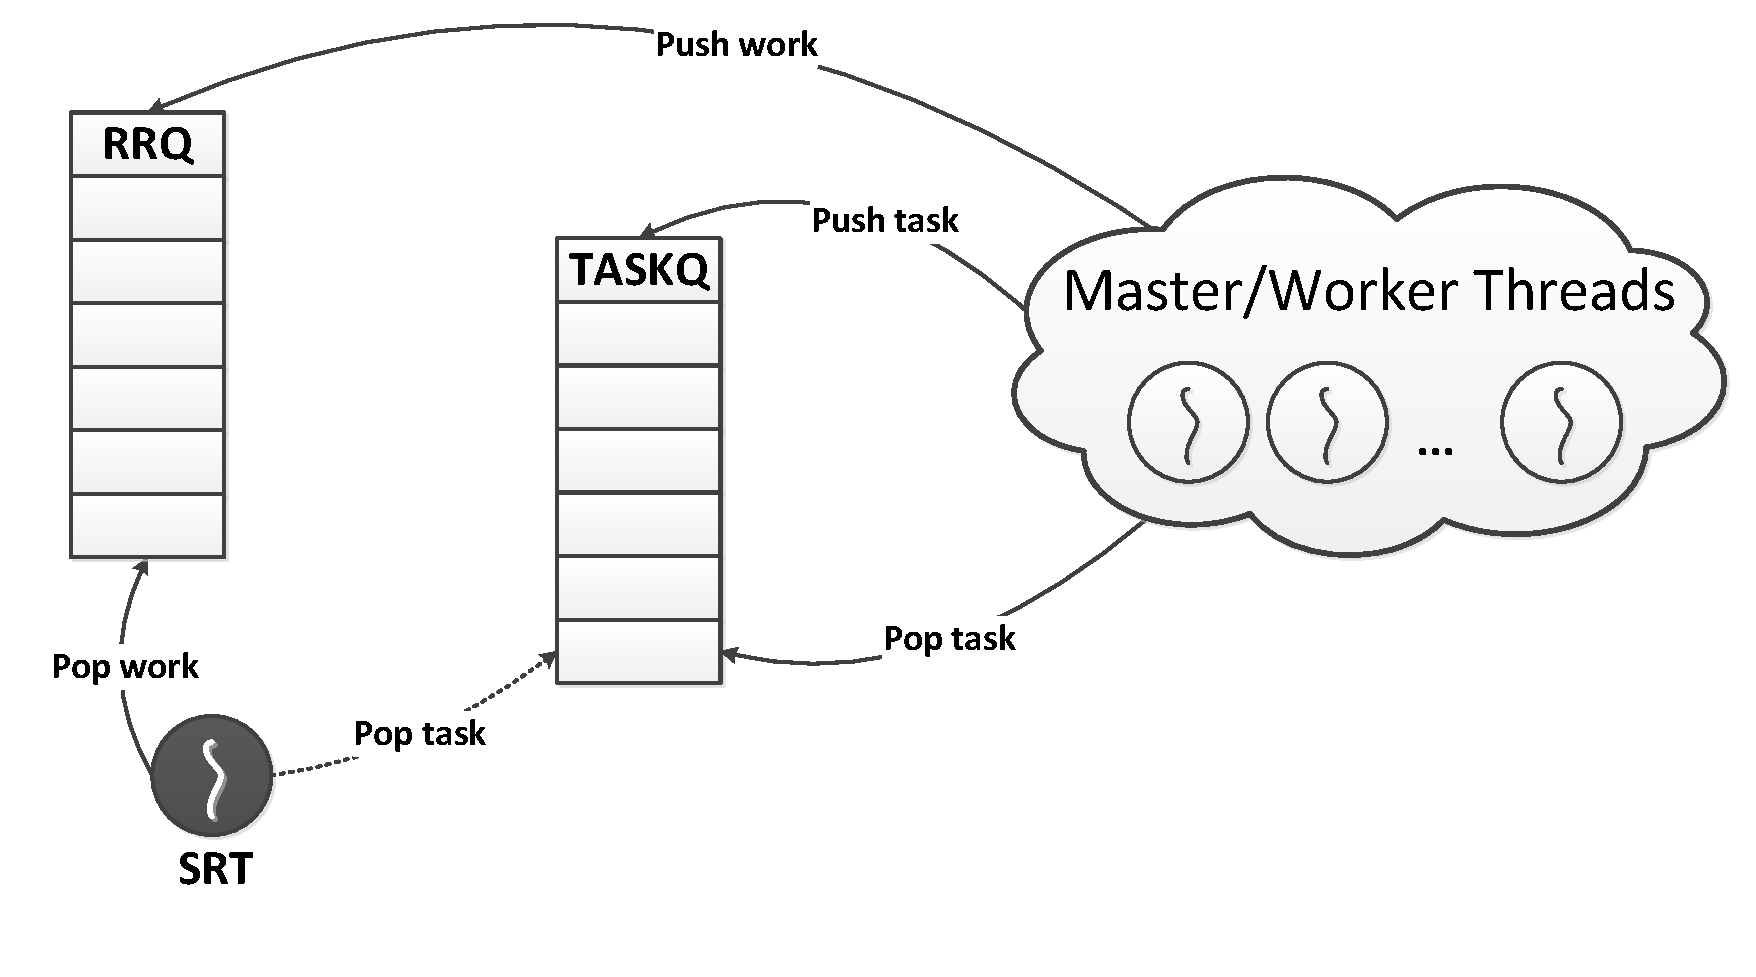
\includegraphics[width=1.0\columnwidth]{Figs/communication.pdf}
	\vspace{-0.5cm}
	\caption{Communication mechanism between master/workers and SRT threads.}
	\label{fig:communication}%
	\vspace{-0.3cm}
\end{figure}
At the same time that the master and worker threads are executing tasks, the SRT is looking for \textit{CREATE} requests in the RRQ to execute.
Listing~\ref{SRTloop} shows the code that the SRT is executing until the end of the parallel execution.
The special runtime thread continuously checks whether there are requests in the RRQ (line 3). As long as there is a pending task creation, the SRT executes the task submission and inserts the task in the TDG with a call to the \texttt{executeRequest} (line 4). If at some point the RRQ becomes empty, the SRT checks the number of ready tasks in the ready queue (lines 5, 6) and if the number of ready tasks is greater than \texttt{maxTasks}, which means that the workers are very loaded, it executes the next ready tasks in the queue. 




\section{Asymmetry-aware runtime system}

Having completed the previous steps we plan to combine our implementations of scheduling techniques and runtime thread migration mechanisms and end up with a novel runtime system for asymmetric architectures that offers two levels of adaptability: first is the choice of the appropriate core type for the runtime execution and second is the appropriate scheduling of the tasks on the available cores.

The first step in discovering the appropriate scheduling-migration mechanism combination is to perform experiments of scientific applications using all the possible combinations of migration and scheduling policies as well as use different machine set-ups in terms of numbers of fast and slow cores.
The analysis of these results will show us whether the combining existing implementations is efficient and under what circumstances.
After concluding to the most appropriate mechanism, we will further verify the results on a larger scale, using an HPC machine with a larger number of cores.


\section{Thesis Roadmap}
The Gantt graph below describes the whole plan with the various stages. 
Each stage corresponds to a section of this chapter. 
The literature review process (named Related works in the graph) is a constant activity that lasts the entire course of the PhD.

A part of work for this PhD was conducted before the PhD enrolment.
This work is described in the graph thus the graph starts from September of 2014.
However, as is noted on the graph, the official PhD enrolment is on September of 2015.

The Gantt graph below has been updated with the current status of the publications. 
During this year, we successfully published the Journal of Scheduling policies.
Furthermore we modified improved and submitted the paper "Asymmetric System Analysis" to multiple conferences but none of them has accepted our work so far.
We plan to perform further modifications in the text and resubmit the paper this October.
In addition, we are in progress of writing the paper for the Runtime Thread Migration and submit it in October as well.


~\\ \\ \\
\noindent\resizebox{\textwidth}{!}{
\begin{ganttchart}[vgrid,hgrid, 
today=37,
today offset=.32,
today label=Current Month,
today rule/.style=%
{draw=blue, ultra thick},
milestone label font=\Large,
group label font=\Large,
title label font=\Large,
bar label font=\Large, 
bar/.append style={fill=green!90}]{1}{52}
%\begin{ganttchart}[vgrid,hgrid, group right shift=0, group top shift=0.7, group height=.3, group peaks width={0.2}]{1}{40}
    \gantttitle{2014}{4}
	\gantttitle{2015}{12} 
	\gantttitle{2016}{12} 
	\gantttitle{2017}{12} 
	\gantttitle{2018}{12} \\
	\gantttitlelist{9,...,12}{1} 
	\gantttitlelist{1,...,12}{1}
	\gantttitlelist{1,...,12}{1}
	\gantttitlelist{1,...,12}{1}
	\gantttitlelist{1,...,12}{1} \\
	\ganttbar{Related works}{1}{52}\\
%	\ganttmilestone{PhD enrolment}{12}\\
	\ganttgroup{\textbf{Scheduling Policies}}{1}{19}\\ %1
	\ganttbar{CATS Scheduler}{1}{9} \\ %2
	\ganttmilestone{\textit{CATS paper}}{9}\\ %3
	\ganttlink{elem2}{elem3}
	\ganttbar{Journal for Scheduling Policies}{9}{19}\\ %4
	\ganttmilestone{\textit{Scheduling policies journal}}{31}\\ %5
	\ganttlink{elem4}{elem5}
	\ganttgroup{\textbf{Asymmetric system analysis}}{13}{24}\\ %6
	\ganttbar{Evaluation and Exploration}{13}{18}\\ %7
	\ganttlinkedbar{Paper writing and submission}{19}{24}\\ %8
	\ganttlinkedbar{Paper review and modification}{24}{38}\\%9
	\ganttmilestone{\textit{Exploration paper}}{45}\\ %10
	\ganttlink{elem9}{elem10}
	\ganttgroup{\textbf{Runtime Thread Migration (RTM)}}{21}{31}\\ %10
	\ganttbar{Implementation and Optimization}{21}{25}\\ %11
	\ganttbar{Evaluation}{26}{27}\\ %12
	\ganttbar{Paper writing for RTM}{27}{38}\\ %13
	\ganttmilestone{\textit{Paper for RTM}}{44}\\ %14
	\ganttlink{elem14}{elem15}
	\ganttgroup{\textbf{Asymmetry Aware Runtime (AAR)}}{31}{44}\\ %15
	\ganttbar{Porting schedulers in runtime}{31}{33}\\ %16
	\ganttbar{Experiments and Optimization}{34}{39}\\ %17	
	\ganttbar{Final evaluation of AAR}{40}{42}\\ %18
	\ganttbar{Paper writing for AAR}{42}{44}\\ %19
	\ganttmilestone{\textit{Paper for AAR}}{52}\\ %20
    \ganttlink{elem20}{elem21}	
	\ganttbar{Thesis writing and defense}{45}{52}		
\end{ganttchart}

\if 0
\begin{ganttchart}[vgrid,hgrid,bar/.append style={fill=green!90}]{1}{52}
%\begin{ganttchart}[vgrid,hgrid, group right shift=0, group top shift=0.7, group height=.3, group peaks width={0.2}]{1}{40}
    \gantttitle{2014}{4}
	\gantttitle{2015}{12} 
	\gantttitle{2016}{12} 
	\gantttitle{2017}{12} 
	\gantttitle{2018}{12} \\
	\gantttitlelist{9,...,12}{1} 
	\gantttitlelist{1,...,12}{1}
	\gantttitlelist{1,...,12}{1}
	\gantttitlelist{1,...,12}{1}
	\gantttitlelist{1,...,12}{1} \\
	\ganttbar{Related works}{1}{52}\\
	\ganttmilestone{PhD enrolment}{12}\\
	\ganttgroup{\textbf{Scheduling Policies}}{1}{19}\\ %1
	\ganttbar{CATS Scheduler}{1}{9} \\ %2
	\ganttmilestone{\textit{CATS paper}}{9}\\ %3
	\ganttlink{elem2}{elem3}
	\ganttbar{Journal for Scheduling Policies}{9}{19}\\ %4
	\ganttmilestone{\textit{Scheduling policies journal}}{31}\\ %5
	\ganttlink{elem4}{elem5}
	\ganttgroup{\textbf{Asymmetric system analysis}}{13}{24}\\ %6
	\ganttbar{Evaluation and Exploration}{13}{18}\\ %7
	\ganttlinkedbar{Paper writing and submission}{19}{24}\\ %8
	\ganttmilestone{\textit{Exploration paper}}{26}\\ %9
	\ganttlink{elem8}{elem9}
	\ganttgroup{\textbf{Runtime Thread Migration (RTM)}}{21}{31}\\ %10
	\ganttbar{Implementation and Optimization}{21}{25}\\ %11
	\ganttbar{Evaluation}{26}{27}\\ %12
	\ganttbar{Paper writing for RTM}{27}{31}\\ %13
	\ganttmilestone{\textit{Paper for RTM}}{39}\\ %14
	\ganttlink{elem13}{elem14}
	\ganttgroup{\textbf{Asymmetry Aware Runtime (AAR)}}{31}{44}\\ %15
	\ganttbar{Porting schedulers in runtime}{31}{33}\\ %16
	\ganttbar{Experiments and Optimization}{34}{39}\\ %17	
	\ganttbar{Final evaluation of AAR}{40}{42}\\ %18
	\ganttbar{Paper writing for AAR}{42}{44}\\ %19
	\ganttmilestone{\textit{Paper for AAR}}{52}\\ %20
    \ganttlink{elem19}{elem20}	
	\ganttbar{Thesis writing and defense}{45}{52}	
	
\end{ganttchart}
\fi
}

